\documentclass[12pt, a4paper]{article}
\usepackage[left=2.54cm, right=2.54cm, bottom=2.54cm, top=2.54cm]{geometry}
\linespread{1}
\usepackage{setspace}
\usepackage[utf8]{inputenc}
\usepackage{blindtext}
\usepackage[T1]{fontenc}
\usepackage{xcolor}
\usepackage{amsfonts}
\usepackage{amsmath}
\usepackage{amssymb}
\usepackage{fancyhdr}
\usepackage{tikz}
\usepackage{hyperref}
\setlength{\parskip}{1em}
\setlength{\parindent}{2em}  % hilangkan indentasi paragraf
\pagestyle{fancy}
\fancyhead{}
\fancyfoot{}
\fancyfoot[R]{\thepage}
\renewcommand{\headrulewidth}{2pt}
\renewcommand{\footrulewidth}{2pt}
\usepackage{graphicx}
\usepackage{multicol}
\graphicspath{ {./img/} }
\usepackage{listings}
\lstset{language=C++, % Specify the programming language
        basicstyle=\ttfamily, % Font style
        numbers=left, % Line numbers on the left
        numberstyle=\tiny, % Style of line numbers
        frame=single, % Add a frame around the code
        breaklines=true, % Enable line wrapping
        captionpos=b, % Caption position (bottom)
        tabsize=2, % Tab size
        showstringspaces=false % Don't show spaces in strings
}

\title{Laporan PBO Quiz 1}
\author{5025241134 Gilbran Mahavikia Raja}
\date{\today}

\begin{document}
\maketitle

\section{Soal}
Soal dapat diakses pada link berikut: \\
\url{https://basecamp.eolymp.com/en/problems/10167}\\
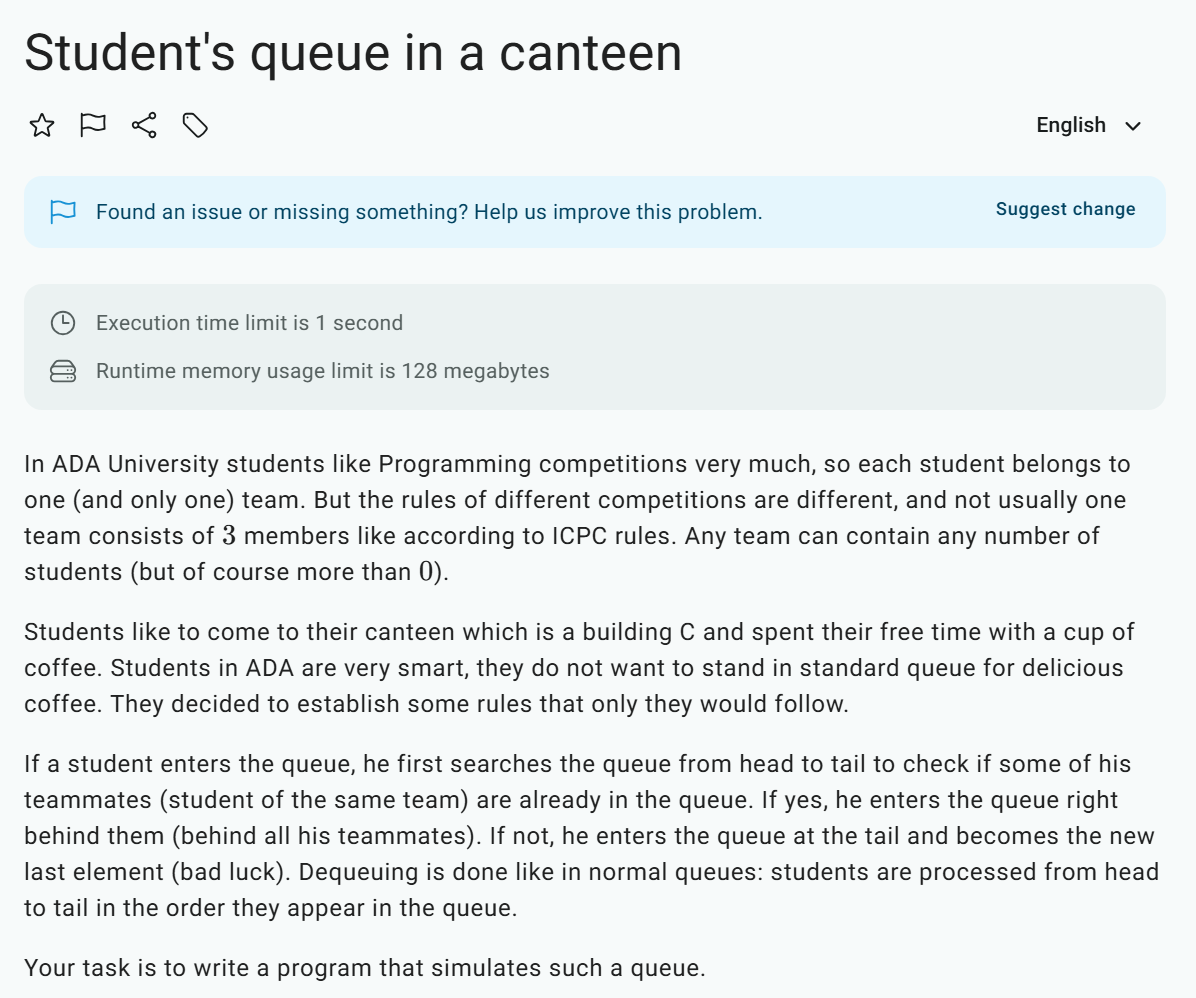
\includegraphics[scale=0.4]{soal.png}

Di ADA University, setiap mahasiswa tergabung dalam satu tim (setiap mahasiswa hanya punya satu tim). Jumlah anggota tiap tim bisa berbeda-beda (tidak harus $3$ seperti aturan ICPC).

Mahasiswa suka nongkrong di kantin dan ingin membeli kopi. Tapi mereka tidak ingin antre seperti biasa. Mereka membuat aturan khusus untuk antrean

\pagebreak
\section{Identifikasi Masalah}

\hspace{2em} Soal ini adalah simulasi antrean khusus berdasarkan kelompok (team queue). Bedanya dengan antrean biasa:

\vspace{-1em}
\begin{itemize}
  \item Bukan hanya FIFO per mahasiswa, tapi juga  mengelompokkan mahasiswa\\ berdasarkan tim.
  \item Jadi, urutannya adalah berdasarkan tim (tim yang sudah masuk duluan tetap di depan tim lain), dan di dalam tim urutannya tetap FIFO.
\end{itemize}
\vspace{-1em}

Input:
\vspace{-1em}
\begin{enumerate}
  \item Angka $t \rightarrow $ jumlah tim.
  \item Untuk setiap tim:
  \item[] \begin{itemize}
    \item Angka $n \rightarrow $ jumlah anggota tim.
    \item Lalu diikuti n ID mahasiswa yang ada di tim itu.
    \item Catatan: setiap mahasiswa punya ID unik ($0$ sampai $10^6$).
    \end{itemize}
  \item Setelah daftar tim, diberikan daftar perintah ("ENQUEUE" $x$ atau "DEQUEUE").
\end{enumerate}
\vspace{-1em}

Output
\vspace{-1em}
\begin{itemize}
  \item Untuk setiap perintah "DEQUEUE", cetak ID mahasiswa yang keluar dari antrean.
\end{itemize}
\vspace{-1em}

Jadi disimpulkan bahwa masalah ini tidak dapat diselesaikan dengan struktur data priority\_queue atau queue biasa, melainkan perlu struktur data tambahan untuk mengelola tim dan anggotanya.

\pagebreak

\section{Solusi dan implementasi pada C++}

\begin{lstlisting}
#include <stdio.h>
#include <queue>
#include <unordered_map>
using namespace std;

int main(){
  int t;
  scanf("%d", &t);

  unordered_map<int, int> team;
  unordered_map<int, queue<int>> members;
  queue<int> torder;
  unordered_map<int, bool> inqueue;

  for (int i = 1; i <= t; i++){
    int n;
    scanf("%d", &n);
    for (int j = 0; j < n; j++){
      int student;
      scanf("%d", &student);
      team[student] = i;
    }
  }

  char cmd[10];
  while (scanf("%s", cmd) != EOF){
    if (cmd[0] == 'E'){
      int ID;
      scanf("%d", &ID);
      int tid = team[ID];
      if (!inqueue[tid]){
        torder.push(tid);
        inqueue[tid] = true;
      }
      members[tid].push(ID);
    }
    else{
      int tid = torder.front();
      int student = members[tid].front();
      members[tid].pop();

      printf("%d\n", student);

      if (members[tid].empty()){
        torder.pop();
        inqueue[tid] = false;
      }
    }
  }
  return 0;
}
\end{lstlisting}

Program ini menyelesaikan masalah \textit{Team Queue}, yaitu simulasi antrean mahasiswa dengan aturan khusus berdasarkan tim. Jika ada mahasiswa dari tim yang sudah berada dalam antrean, maka mahasiswa baru masuk di belakang rekannya, bukan di antrean global langsung.

Untuk menyelesaikan masalah ini, digunakan beberapa struktur data. Pertama, \texttt{unordered\_map<int,int> team} yang memetakan setiap mahasiswa ke timnya, sehingga pencarian tim dari student ID cepat dilakukan. Kedua, \texttt{unordered\_map<int,queue<int>> members} yang menyimpan antrean mahasiswa per tim, agar urutan masuk dan keluar anggota tim tetap FIFO. Ketiga, \texttt{queue<int> torder} yang menyimpan urutan tim di antrean global, sehingga proses "DEQUEUE" dapat mengikuti giliran tim. Terakhir, \texttt{unordered\_map<int,bool> inqueue} dipakai sebagai penanda apakah sebuah tim sudah ada di antrean global, supaya tidak masuk dua kali.

Logikanya sederhana: saat "ENQUEUE", mahasiswa ditambahkan ke antrean timnya, dan jika tim belum ada di antrean global maka tim ditambahkan ke torder. Saat "DEQUEUE", mahasiswa dari tim paling depan diproses, jika antrean tim kosong, tim tersebut dikeluarkan dari torder. Dengan kombinasi struktur data ini, setiap operasi dapat dilakukan dengan cepat, sambil tetap memenuhi aturan khusus antrean berdasarkan tim.

Dan terakhir, gunakan pendekatan C saat proses input dan output untuk efisiensi. Karena ketika saya coba menggunakan C++ STL \texttt{cin} dan \texttt{cout}, program saya tidak memenuhi syarat memory yaitu 0.30mb dan ketika menggunakan \texttt{scanf} dan \texttt{printf}, program saya dapat memenuhi syarat tersebut.

\pagebreak

\section{Bukti}
Berikut adalah bukti bahwa solusi saya mendapatkan verdict \textbf{Accepted}, time \textbf{1ms}, dan memory \textbf{0.30mb}.\\
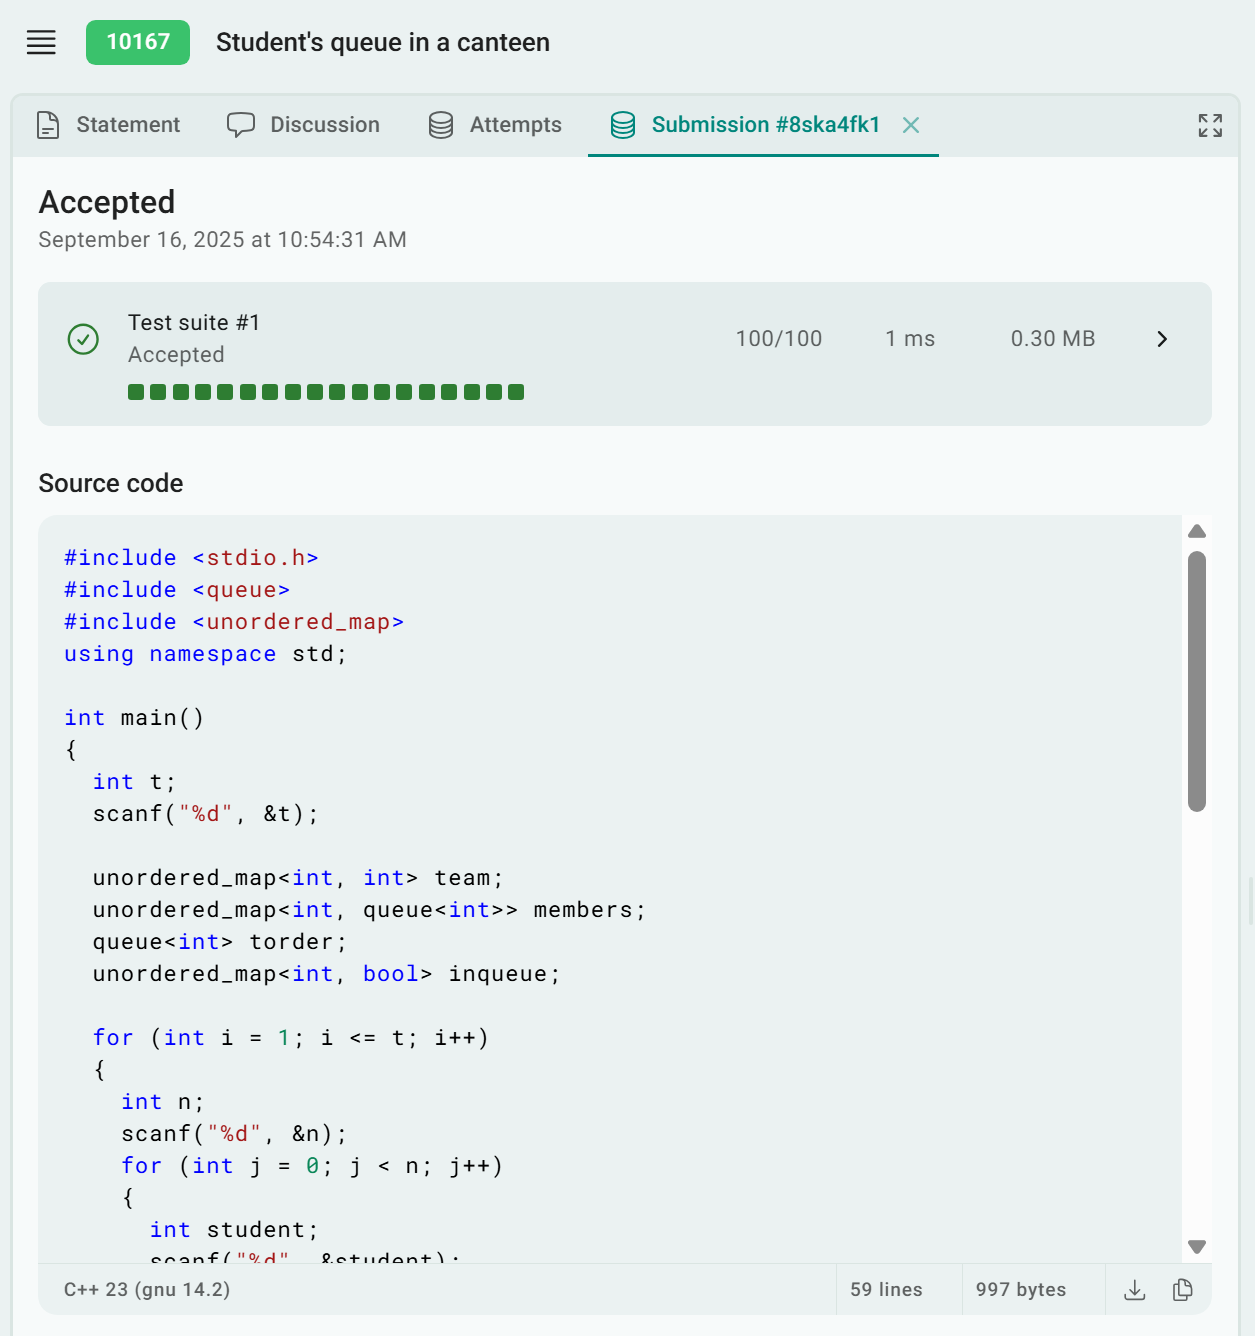
\includegraphics[scale=0.4]{bukti.png}
\end{document}